

\tikzset{every picture/.style={line width=0.75pt}} %set default line width to 0.75pt        
\begin{center}
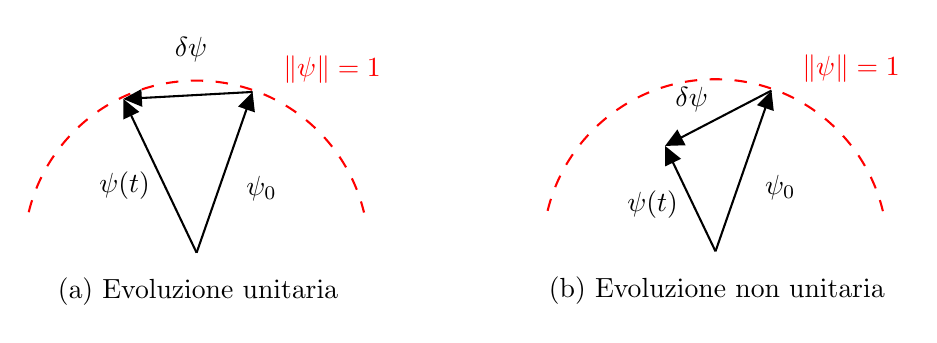
\begin{tikzpicture}[x=0.75pt,y=0.75pt,yscale=-1,xscale=1]
%uncomment if require: \path (0,300); %set diagram left start at 0, and has height of 300

%Straight Lines [id:da13244260408452746] 
\draw    (192.71,166.46) -- (219.01,90.89) ;
\draw [shift={(219.67,89)}, rotate = 469.19] [fill={rgb, 255:red, 0; green, 0; blue, 0 }  ][line width=0.75]  [draw opacity=0] (8.93,-4.29) -- (0,0) -- (8.93,4.29) -- cycle    ;

%Shape: Arc [id:dp47261095341946513] 
\draw  [draw opacity=0][dash pattern={on 4.5pt off 4.5pt}] (111.82,146.94) .. controls (120.55,110.84) and (152.96,83.88) .. (191.85,83.54) .. controls (231.29,83.2) and (264.56,110.36) .. (273.36,147.09) -- (192.57,166.46) -- cycle ; \draw  [color={rgb, 255:red, 255; green, 0; blue, 0 }  ,draw opacity=1 ][dash pattern={on 4.5pt off 4.5pt}] (111.82,146.94) .. controls (120.55,110.84) and (152.96,83.88) .. (191.85,83.54) .. controls (231.29,83.2) and (264.56,110.36) .. (273.36,147.09) ;
%Straight Lines [id:da4640817340211536] 
\draw    (192.71,166.46) -- (158.26,94.2) ;
\draw [shift={(157.4,92.39)}, rotate = 424.51] [fill={rgb, 255:red, 0; green, 0; blue, 0 }  ][line width=0.75]  [draw opacity=0] (8.93,-4.29) -- (0,0) -- (8.93,4.29) -- cycle    ;

%Straight Lines [id:da676932203344851] 
\draw    (219.67,89) -- (159.4,92.29) ;
\draw [shift={(157.4,92.39)}, rotate = 356.88] [fill={rgb, 255:red, 0; green, 0; blue, 0 }  ][line width=0.75]  [draw opacity=0] (8.93,-4.29) -- (0,0) -- (8.93,4.29) -- cycle    ;

%Straight Lines [id:da439787380235227] 
\draw    (442.71,165.79) -- (469.01,90.22) ;
\draw [shift={(469.67,88.33)}, rotate = 469.19] [fill={rgb, 255:red, 0; green, 0; blue, 0 }  ][line width=0.75]  [draw opacity=0] (8.93,-4.29) -- (0,0) -- (8.93,4.29) -- cycle    ;

%Shape: Arc [id:dp10305939137664444] 
\draw  [draw opacity=0][dash pattern={on 4.5pt off 4.5pt}] (361.82,146.27) .. controls (370.55,110.17) and (402.96,83.21) .. (441.85,82.87) .. controls (481.29,82.53) and (514.56,109.69) .. (523.36,146.43) -- (442.57,165.79) -- cycle ; \draw  [color={rgb, 255:red, 255; green, 0; blue, 0 }  ,draw opacity=1 ][dash pattern={on 4.5pt off 4.5pt}] (361.82,146.27) .. controls (370.55,110.17) and (402.96,83.21) .. (441.85,82.87) .. controls (481.29,82.53) and (514.56,109.69) .. (523.36,146.43) ;
%Straight Lines [id:da4447134676498914] 
\draw    (442.71,165.79) -- (419.26,116.8) ;
\draw [shift={(418.4,115)}, rotate = 424.41999999999996] [fill={rgb, 255:red, 0; green, 0; blue, 0 }  ][line width=0.75]  [draw opacity=0] (8.93,-4.29) -- (0,0) -- (8.93,4.29) -- cycle    ;

%Straight Lines [id:da8691059971533945] 
\draw    (469.67,88.33) -- (420.17,114.08) ;
\draw [shift={(418.4,115)}, rotate = 332.52] [fill={rgb, 255:red, 0; green, 0; blue, 0 }  ][line width=0.75]  [draw opacity=0] (8.93,-4.29) -- (0,0) -- (8.93,4.29) -- cycle    ;


% Text Node
\draw (158,134) node   {$\psi ( t)$};
% Text Node
\draw (224,135.6) node   {$\psi _{0}$};
% Text Node
\draw (190,68.4) node   {$\delta \psi $};
% Text Node
\draw (258,78.2) node [color={rgb, 255:red, 255; green, 0; blue, 0 }  ,opacity=1 ]  {$\| \psi \| =1$};
% Text Node
\draw (193.33,185.33) node  [align=left] {(a) Evoluzione unitaria};
% Text Node
\draw (412.4,143.33) node   {$\psi ( t)$};
% Text Node
\draw (474,134.93) node   {$\psi _{0}$};
% Text Node
\draw (431.2,92.8) node   {$\delta \psi $};
% Text Node
\draw (508,77.53) node [color={rgb, 255:red, 255; green, 0; blue, 0 }  ,opacity=1 ]  {$\| \psi \| =1$};
% Text Node
\draw (443.33,184.67) node  [align=left] {(b) Evoluzione non unitaria};


\end{tikzpicture}
\end{center}